\chapter{About split, interval and permutation graphs}
\label{sec:25}

\abstract*{}

\abstract{}

%%%%%%%% draft version
% uncomment for final version
\tableofcontents


\section{A multiply perfect graph}
\label{sec:25.1}

Following Martin Golumbic (see \citep{GOL-2004} p. 149), we call a given graph g:
\begin{itemize}
\item \emph{Comparability} graph when $g$  is \emph{transitively orientable};
\item \emph{Triangulated} graph when $g$ does not contain any \emph{chordless cycle} of length 4 and more;
\item \emph{Interval} graph when $g$ is \emph{triangulated} and its dual $-g$ is a \emph{comparability} graph;
\item \emph{Permutation} graph when $g$ and its dual $-g$ bothe are \emph{comparability} graphs;
\item \emph{Split} graph when $g$ and its dual $-g$ bothe are \emph{triangulated} graphs.
\end{itemize}

To illustrate these \emph{perfect} graph classes, we will generate from 8 intervals, randomly chosen in the default integer range $[0,10]$, a \emph{RandomIntervalIntersectionsGraph} instance $g$ (see Line 2 below). 
\begin{lstlisting}
>>> from graphs import\
...          RandomIntervalIntersectionsGraph
>>> g = RandomIntervalIntersectionsGraph(\
...                          order=8,seed=100)
>>> g
 *------- Graph instance description ------*
  Instance class   : RandomIntervalIntersectionsGraph
  Instance name    : randIntervalIntersections
  Seed             : 100
  Graph Order      : 8
  Graph Size       : 23
  Valuation domain : [-1.0; 1.0]
  Attributes       : ['seed', 'name', 'order',
        'intervals', 'vertices', 'valuationDomain',
        'edges', 'size', 'gamma']
>>> print(g.intervals)
  [(2,7),(2,7),(5,6),(6,8),(1,8),(1,1),(4,7),(0,10)]
\end{lstlisting}

With \texttt{seed = 100}, we obtain here an interval graph, in fact apperfect graph, which is \emph{conjointly} a triangulated, a comparability, a split and a permutation graph (see Listing \ref{list:25.1} Lines 6, 10, 14).
\begin{lstlisting}[caption={Testing perfect graph categories.},label=list:25.1,basicstyle=\scriptsize]
>>> g.isPerfectGraph(Comments=True)
  Graph randIntervalIntersections is perfect !
>>> g.isIntervalGraph(Comments=True)
  Graph 'randIntervalIntersections' is triangulated.
  Graph 'dual_randIntervalIntersections' is transitively orientable.
  => Graph 'randIntervalIntersections' is an interval graph.
>>> g.isSplitGraph(Comments=True)
  Graph 'randIntervalIntersections' is triangulated.
  Graph 'dual_randIntervalIntersections' is triangulated.
  => Graph 'randIntervalIntersections' is a split graph.
>>> g.isPermutationGraph(Comments=True)
  Graph 'randIntervalIntersections' is transitively orientable.
  Graph 'dual_randIntervalIntersections' is transitively orientable.
  => Graph 'randIntervalIntersections' is a permutation graph.
>>> print(g.computePermutation())
  ['v5', 'v6', 'v4', 'v2', 'v1', 'v3', 'v7', 'v8']
  ['v8', 'v6', 'v1', 'v2', 'v3', 'v4', 'v7', 'v5']
  [8, 2, 6, 5, 7, 4, 3, 1]
>>> g.exportGraphViz('randomSplitGraph')
  *---- exporting a dot file for GraphViz tools ---------*
   Exporting to randomSplitGraph.dot
   fdp -Tpng randomSplitGraph.dot -o randomSplitGraph.png
\end{lstlisting}
\begin{figure}[h]
\sidecaption
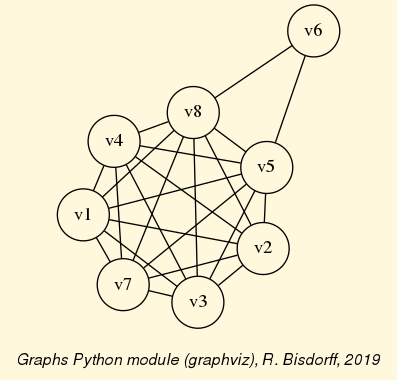
\includegraphics[width=6cm]{Figures/randomSplitGraph.png}
\caption{A conjointly triangulated, comparability, interval, permutation and split graph} 
\label{fig:25.1}       % Give a unique label
\end{figure}

In Fig. \ref{fig:25.1} we may readily recognize the essential characteristic of split graphs, namely being always splitable into two disjoint sub-graphs: an \emph{independent choice} {'v6'} and a \emph{clique} \{'v1', 'v2', 'v3', 'v4', 'v5', 'v7', 'v8'\}; which explains their name.

Notice however that the four properties:
\begin{enumerate}
\item $g$ is a \emph{comparability} graph;
\item $g$ is a \emph{co-comparability} graph, i.e. $-g$ is a comparability graph;
\item $g$ is a \emph{triangulated} graph;
\item $g$ is a \emph{co-triangulated} graph, i.e. $-g$ is a comparability graph;
\end{enumerate}
are independent of one another (see \citep{GOL-2004} p. 275).

\section{Who is the liar?}
\label{sec:25.2}


Claude \Berge's famous mystery story (see \citep{GOL-2004} p.20) may well illustrate the importance of being an \emph{interval} graph.

Suppose the file \texttt{berge.py} \footnote{A \texttt{Graph} encoded file \texttt{berge.py} may be found in the \texttt{examples} directory of the \Digraph resources.} contains the following \texttt{Graph} instance data:
\begin{lstlisting}
  vertices = {
    'A': {'name': 'Abe', 'shortName': 'A'},
    'B': {'name': 'Burt', 'shortName': 'B'},
    'C': {'name': 'Charlotte', 'shortName': 'C'},
    'D': {'name': 'Desmond', 'shortName': 'D'},
    'E': {'name': 'Eddie', 'shortName': 'E'},
    'I': {'name': 'Ida', 'shortName': 'I'},
    }
  valuationDomain = {'min':-1,'med':0,'max':1}
  edges = {
    frozenset(['A','B']) : 1, 
    frozenset(['A','C']) : -1, 
    frozenset(['A','D']) : 1, 
    frozenset(['A','E']) : 1, 
    frozenset(['A','I']) : -1, 
    frozenset(['B','C']) : -1, 
    frozenset(['B','D']) : -1, 
    frozenset(['B','E']) : 1, 
    frozenset(['B','I']) : 1, 
    frozenset(['C','D']) : 1, 
    frozenset(['C','E']) : 1, 
    frozenset(['C','I']) : 1, 
    frozenset(['D','E']) : -1, 
    frozenset(['D','I']) : 1, 
    frozenset(['E','I']) : 1, 
    }
\end{lstlisting}

Six professors (labeled 'A', 'B', 'C', 'D', 'E' and 'I') had been to the library on the day that a rare tractate was stolen. Each entered once, stayed for some time, and then left. If two professors were in the library at the same time, then at least one of them saw the other. Detectives questioned the professors and gathered the testimonies that 'A' saw 'B' and 'E'; 'B' saw 'A' and 'I'; 'C' saw 'D' and 'I'; 'D' saw 'A' and 'I'; 'E' saw 'B' and 'I'; and 'I' saw 'C' and 'E'. This data is gathered in the previous file, where each positive edge $\{x,y\}$ models the testimony that, either $x$ saw $y$, or $y$ saw $x$.
\begin{lstlisting}
>>> from graphs import Graph
>>> g = Graph('berge')
>>> g.showShort()
  *---- short description of the graph ----*
   Name             : 'berge'
   Vertices         :  ['A', 'B', 'C', 'D', 'E', 'I']
   Valuation domain :  {'min': -1, 'med': 0, 'max': 1}
   Gamma function   : 
    A -> ['D', 'B', 'E']
    B -> ['E', 'I', 'A']
    C -> ['E', 'D', 'I']
    D -> ['C', 'I', 'A']
    E -> ['C', 'B', 'I', 'A']
    I -> ['C', 'E', 'B', 'D']
>>> g.exportGraphViz('berge1')
  *---- exporting a dot file for GraphViz tools ---------*
   Exporting to berge1.dot
   fdp -Tpng berge1.dot -o berge1.png
\end{lstlisting}
\begin{figure}[h]
\sidecaption
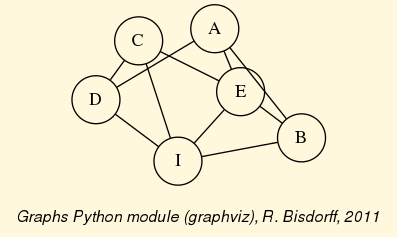
\includegraphics[width=6cm]{Figures/berge1.png}
\caption{Graph representation of the testimonies of the professors} 
\label{fig:25.2}       % Give a unique label
\end{figure}

From graph theory we know that time interval intersections graphs must in fact be interval graphs, i.e. \emph{triangulated} and \emph{co-comparative} graphs. The testimonies graph should therefore not contain any chordless cycle of four and more vertices. Now, the presence or not of such chordless cycles in the testimonies graph may be checked as follows:
\begin{lstlisting}
>>> g.computeChordlessCycles()
  Chordless cycle certificate: ['D','C','E','A','D']
  Chordless cycle certificate: ['D','I','E','A','D']
  Chordless cycle certificate: ['D','I','B','A','D']
  [(['D','C','E','A','D'],frozenset({'C','D','E','A'})),
  (['D','I','E','A','D'],frozenset({'D','E','I','A'})),
  (['D','I','B','A','D'],frozenset({'D','B','I','A'}))]
\end{lstlisting}
We see in the Listing above three intersection cycles of length 4, which is impossible to occur on the linear time line. Obviously one professor lied!

And it is $D$ ; if we put to doubt his testimony that he saw 'A' (see Line 1 below), we obtain indeed a triangulated graph instance whose dual is a comparability graph.
\begin{lstlisting}
>>> g.setEdgeValue( ('D','A'), 0)
>>> g.showShort()
  *---- short description of the graph ----*
   Name             : 'berge'
   Vertices         :  ['A','B','C','D','E','I']
   Valuation domain :  {'med': 0,'min': -1,'max': 1}
   Gamma function   : 
    A -> ['B', 'E']
    B -> ['A', 'I', 'E']
    C -> ['I', 'E', 'D']
    D -> ['I', 'C']
    E -> ['A', 'I', 'B', 'C']
    I -> ['B', 'E', 'D', 'C']
>>> g.isIntervalGraph(Comments=True)
  Graph 'berge' is triangulated.
  Graph 'dual_berge' is transitively orientable.
  => Graph 'berge' is an interval graph.
>>> g.exportGraphViz('berge2')
  *---- exporting a dot file for GraphViz tools ---------*
   Exporting to berge2.dot
   fdp -Tpng berge2.dot -o berge2.png
\end{lstlisting}
\begin{figure}[h]
\sidecaption
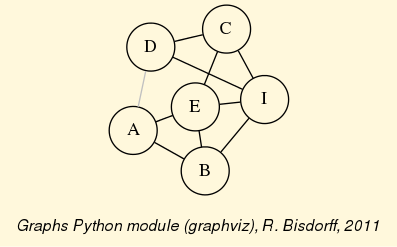
\includegraphics[width=6cm]{Figures/berge2.png}
\caption{The triangulated testimonies graph} 
\label{fig:25.3}       % Give a unique label
\end{figure}

\section{Generating permutation graphs}
\label{sec:25.3}

A graph is called a \emph{permutation} or \emph{inversion} graph if there exists a permutation of its list of vertices such that the graph is isomorphic to the inversions operated by the permutation in this list (see \citep{GOL-2004} Chapter 7, pp 157-170). This kind is also part of the class of perfect graphs.
\begin{lstlisting}
>>> from graphs import PermutationGraph
>>> g = PermutationGraph(permutation = [4,3,6,1,5,2])
>>> g
  *------- Graph instance description ------*
   Instance class   : PermutationGraph
   Instance name    : permutationGraph
   Graph Order      : 6
   Permutation      : [4, 3, 6, 1, 5, 2]
   Graph Size       : 9
   Valuation domain : [-1.00; 1.00]
   Attributes       : ['name', 'vertices', 'order',
                  'permutation', 'valuationDomain',
                  'edges', 'size', 'gamma']
>>> g.isPerfectGraph()
  True
>>> g.exportGraphViz()
  *---- exporting a dot file for GraphViz tools ---------*
   Exporting to permutationGraph.dot
   fdp -Tpng permutationGraph.dot\
       -o permutationGraph.png
\end{lstlisting}
\begin{figure}[h]
\sidecaption
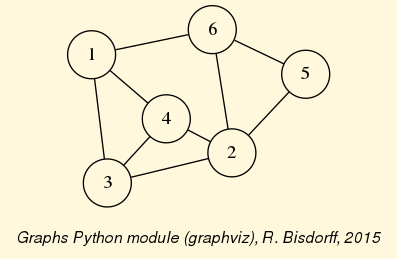
\includegraphics[width=6cm]{Figures/permutationGraph.png}
\caption{The default \Digraph permutation graph} 
\label{fig:25.4}       % Give a unique label
\end{figure}

By using color sorting queues, the minimal vertex coloring for a permutation graph is computable in $O\big(n log(n)\big)$ (see \citep{GOL-2004}).
\begin{lstlisting}
>>> g.computeMinimalVertexColoring(Comments=True)
    vertex 1: lightcoral
    vertex 2: lightcoral
    vertex 3: lightblue
    vertex 4: gold
    vertex 5: lightblue
    vertex 6: gold
>>> g.exportGraphViz(fileName='coloredPermutationGraph',\
...                  WithVertexColoring=True)
  *---- exporting a dot file for GraphViz tools -------*
   Exporting to coloredPermutationGraph.dot
   fdp -Tpng coloredPermutationGraph.dot\
       -o coloredPermutationGraph.png
\end{lstlisting}
\begin{figure}[h]
\sidecaption
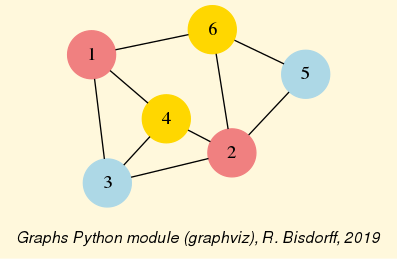
\includegraphics[width=6cm]{Figures/coloredPermutationGraph.png}
\caption{Minimal vertex coloring of the permutation graph.} 
\label{fig:25.5}       % Give a unique label
\end{figure}

The correspondingly colored \emph{matching diagram} of the nine inversions --the actual edges of the permutation graph--, which are induced by the given [4,3,6,1,5,2] permutation, may as well be drawn with the graphviz \texttt{neato} layout and explicitly positioned horizontal lists of vertices (see Fig. \ref{fig:25.6}).
\begin{lstlisting}
>>> g.exportPermutationGraphViz(\
...                    WithEdgeColoring=True)
  *---- exporting a dot file for GraphViz tools ------*
   Exporting to perm_permutationGraph.dot
   neato -n -Tpng perm_permutationGraph.dot\
            -o perm_permutationGraph.png
\end{lstlisting}
\begin{figure}[h]
\sidecaption
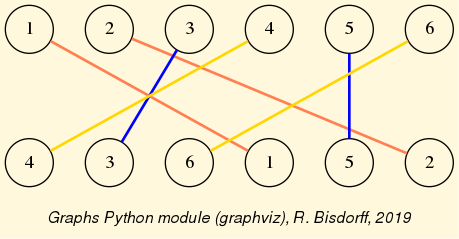
\includegraphics[width=8cm]{Figures/perm_permutationGraph.png}
\caption{Colored matching diagram of the permutation [4,3,6,1,5,2].} 
\label{fig:25.6}       % Give a unique label
\end{figure}

As mentioned before, a permutation graph and its dual are \emph{transitively orientable}. The \texttt{transitiveOrientation()} method constructs from a given permutation graph a digraph where each edge of the permutation graph is converted into an arc oriented in increasing alphabetic order of the adjacent vertices' keys (see \citep{GOL-2004}). This orientation of the edges of a permutation graph is always transitive and delivers a \emph{transitive ordering} of the vertices.
\begin{lstlisting}
>>> dg = g.transitiveOrientation()
>>> dg
  *------- Digraph instance description ------*
   Instance class   : TransitiveDigraph
   Instance name    : oriented_permutationGraph
   Digraph Order      : 6
   Digraph Size       : 9
   Valuation domain : [-1.00; 1.00]
   Determinateness  : 100.000
   Attributes       : ['name', 'order', 'actions',
                    'valuationdomain', 'relation',
                    'gamma', 'notGamma', 'size']
>>> print('Transitivity degree: %.3f' %\
...          dgd.computeTransitivityDegree() ) 
   Transitivity degree: 1.000
>>> dg.exportGraphViz(fileName='orientedPermGraph')
  *---- exporting a dot file for GraphViz tools -----*
   Exporting to orientedPermGraph.dot
   dot -Grankdir=TB -Tpng orientedPermGraph.dot\
                    -o orientedPermGraph.png
\end{lstlisting}
\begin{figure}[h]
\sidecaption
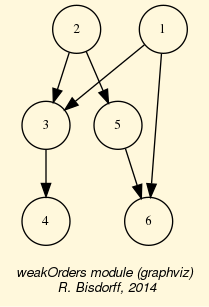
\includegraphics[width=6cm]{Figures/oriented_permutationGraph.png}
\caption{The transitive orientation of the permutation graph.} 
\label{fig:25.7}       % Give a unique label
\end{figure}

The dual of a permutation graph is again a permutation graph and as such also transitively orientable.
\begin{lstlisting}
>>> dgd = (-g).transitiveOrientation()
>>> print('Dual transitivity degree: %.3f' %\
...            dgd.computeTransitivityDegree() )
   Dual transitivity degree: 1.00
\end{lstlisting}

\section{Recognizing permutation graphs}
\label{sec:25.4}

Now, a given graph $g$ is a permutation graph if and only if both $g$ \textbf{and} $-g$ are transitively orientable. This  property gives a polynomial test procedure (in $O(n^3)$ due to the transitivity check) for recognizing permutation graphs.

Let us consider, for instance, the following random graph of order 8 generated with an edge probability of $40\%$ and a random seed equal to $4335$.
\begin{lstlisting}
>>> from graphs import RandomGraph
>>> g = RandomGraph(order=8,\
...                 edgeProbability=0.4,seed=4335)
>>> g
  *------- Graph instance description ------*
   Instance class   : RandomGraph
   Instance name    : randomGraph
   Seed             : 4335
   Edge probability : 0.4
   Graph Order      : 8
   Graph Size       : 10
   Valuation domain : [-1.00; 1.00]
   Attributes       : ['name', 'order', 'vertices',
                       'valuationDomain', 'seed',
                       'edges', 'size', 'gamma',
                       'edgeProbability']
>>> g.isPerfectGraph()
  True
>>> g.exportGraphViz()
\end{lstlisting}		    
\begin{figure}[h]
\sidecaption
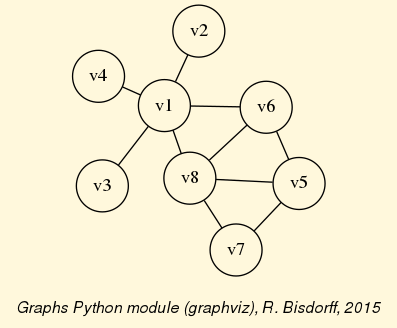
\includegraphics[width=6cm]{Figures/randomGraph4335.png}
\caption{Random graph of order 8 generated with edge probability $0.4$.} 
\label{fig:25.8}       % Give a unique label
\end{figure}

If the random perfect graph instance $g$, shown in Fig. \ref{fig:25.8}, is indeed a permutation graph, $g$ and its dual $-g$ should be \emph{transitively orientable}, i.e. comparability graphs (see \citep{GOL-2004}). With the \texttt{isComparabilityGraph()} test, we may easily check this fact. This method proceeds indeed by trying to construct a transitive neighbourhood decomposition of a given graph instance and, if successful, stores the resulting edge orientations into a \texttt{edgeOrientations} attribute (see \citep{GOL-2004} p.129-132).
\begin{lstlisting}[basicstyle=\scriptsize]
>>> if g.isComparabilityGraph():
...     print(g.edgeOrientations)  
 {('v1','v1'): 0, ('v1','v2'): 1, ('v2','v1'): -1, ('v1','v3'): 1,
  ('v3','v1'): -1, ('v1','v4'): 1, ('v4','v1'): -1, ('v1','v5'): 0,
  ('v5','v1'): 0, ('v1','v6'): 1, ('v6','v1'): -1, ('v1','v7'): 0,
  ('v7','v1'): 0, ('v1','v8'): 1, ('v8','v1'): -1, ('v2','v2'): 0,
  ('v2','v3'): 0, ('v3','v2'): 0, ('v2','v4'): 0, ('v4','v2'): 0,
  ('v2','v5'): 0, ('v5','v2'): 0, ('v2','v6'): 0, ('v6','v2'): 0,
  ('v2','v7'): 0, ('v7','v2'): 0, ('v2','v8'): 0, ('v8','v2'): 0,
  ('v3','v3'): 0, ('v3','v4'): 0, ('v4','v3'): 0, ('v3','v5'): 0,
  ('v5','v3'): 0, ('v3','v6'): 0, ('v6','v3'): 0, ('v3','v7'): 0,
  ('v7','v3'): 0, ('v3','v8'): 0, ('v8','v3'): 0, ('v4','v4'): 0,
  ('v4','v5'): 0, ('v5','v4'): 0, ('v4','v6'): 0, ('v6','v4'): 0,
  ('v4','v7'): 0, ('v7','v4'): 0, ('v4','v8'): 0, ('v8','v4'): 0,
  ('v5','v5'): 0, ('v5','v6'): 1, ('v6','v5'): -1, ('v5','v7'): 1,
  ('v7','v5'): -1, ('v5','v8'): 1, ('v8','v5'): -1, ('v6','v6'): 0,
  ('v6','v7'): 0, ('v7','v6'): 0, ('v6','v8'): 1, ('v8','v6'): -1,
  ('v7','v7'): 0, ('v7','v8'): 1, ('v8','v7'): -1, ('v8','v8'): 0}
\end{lstlisting}		    
\begin{figure}[h]
\sidecaption
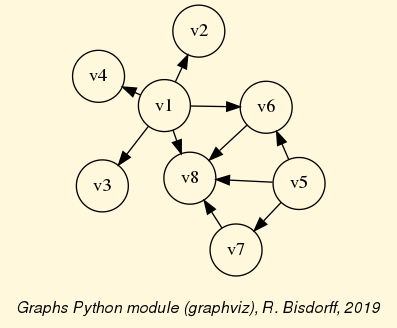
\includegraphics[width=7cm]{Figures/transOrientGraph.png}
\caption{Transitive neighbourhoods of the graph $g$.} 
\label{fig:25.9}       % Give a unique label
\end{figure}

The resulting orientation of the edges of $g$, shown in Fig. \ref{fig:25.9}, is indeed transitive. The same procedure applied to the dual graph $gd = -g$ gives as well a transitive orientation to the edges of $-g$.

.. code-block:: pycon
   :linenos:

\begin{lstlisting}[basicstyle=\scriptsize]
>>> gd = -g
>>> if gd.isComparabilityGraph():
...     print(gd.edgeOrientations) 
  {('v1','v1'): 0, ('v1','v2'): 0, ('v2','v1'): 0, ('v1','v3'): 0,
   ('v3','v1'): 0, ('v1','v4'): 0, ('v4','v1'): 0, ('v1','v5'): 1,
   ('v5','v1'): -1, ('v1','v6'): 0, ('v6','v1'): 0, ('v1','v7'): 1,
   ('v7','v1'): -1, ('v1','v8'): 0, ('v8','v1'): 0, ('v2','v2'): 0,
   ('v2','v3'): -2, ('v3','v2'): 2, ('v2','v4'): -3, ('v4','v2'): 3,
   ('v2','v5'): 1, ('v5','v2'): -1, ('v2','v6'): 1, ('v6','v2'): -1,
   ('v2','v7'): 1, ('v7','v2'): -1, ('v2','v8'): 1, ('v8','v2'): -1,
   ('v3','v3'): 0, ('v3','v4'): -3, ('v4','v3'): 3, ('v3','v5'): 1,
   ('v5','v3'): -1, ('v3','v6'): 1, ('v6','v3'): -1, ('v3','v7'): 1,
   ('v7','v3'): -1, ('v3','v8'): 1, ('v8','v3'): -1, ('v4','v4'): 0,
   ('v4','v5'): 1, ('v5','v4'): -1, ('v4','v6'): 1, ('v6','v4'): -1,
   ('v4','v7'): 1, ('v7','v4'): -1, ('v4','v8'): 1, ('v8','v4'): -1,
   ('v5','v5'): 0, ('v5','v6'): 0, ('v6','v5'): 0, ('v5','v7'): 0,
   ('v7','v5'): 0, ('v5','v8'): 0, ('v8','v5'): 0, ('v6','v6'): 0,
   ('v6','v7'): 1, ('v7','v6'): -1, ('v6','v8'): 0, ('v8','v6'): 0,
   ('v7','v7'): 0, ('v7','v8'): 0, ('v8','v7'): 0, ('v8','v8'): 0}
\end{lstlisting}
\begin{figure}[h]
\sidecaption
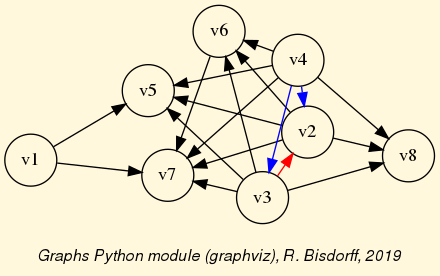
\includegraphics[width=7cm]{Figures/transOrientDualGraph.png}
\caption{Transitive neighbourhoods of the dual graph $-g$. It is worthwhile noticing that the orientation of $g$ is achieved with a single neighbourhood decomposition, covering all the vertices. Whereas, the orientation of the dual graph $-g$ here needs a decomposition into three subsequent neighbourhoods marked in black, red and blue.} 
\label{fig:25.10}       % Give a unique label
\end{figure}
 
Let us recheck these facts by explicitly constructing transitively oriented digraph instances with the \texttt{computeTransitivelyOrientedDigraph()} method \footnote{The \texttt{PartiallyDetermined = True} flag (see Lines 2 and 7 above) is required here in order to orient only the actual edges of the graphs. Relations between vertices not linked by an edge are put to the indeterminate characteristic value $0$. This allows us to compute, later on, convenient disjunctive digraph fusions.
}. 
\begin{lstlisting}
>>> og = g.computeTransitivelyOrientedDigraph(\
...                      PartiallyDetermined = )
>>> print('Transitivity degree: %.3f' %\
...                      (og.transitivityDegree)) 
  Transitivity degree: 1.000
>>> ogd = (-g).computeTransitivelyOrientedDigraph(\
...                      PartiallyDetermined = True)
>>> print('Transitivity degree: %.3f' %\
...                      (ogd.transitivityDegree)) 
  Transitivity degree: 1.000
\end{lstlisting}

As both graphs are indeed transitively orientable (see Lines 5 and 10 above), we may conclude that the given random graph $g$ is actually a permutation graph instance. Yet, we still need to find now its corresponding permutation. We therefore implement a recipee given by Martin Golumbic \citep{GOL-2004} p.159.

We will first \emph{fuse} both $og$ and $ogd$ orientations above with an \emph{epistemic disjunction} operated with the symmetric \texttt{o-max} operator (see Section \ref{sec:2.5}).
\begin{lstlisting}
>>> from digraphs import FusionDigraph
>>> f1 = FusionDigraph(og,ogd,operator='o-max')
>>> s1 = f1.computeCopelandRanking()
>>> print(s1)
  ['v5','v7','v1','v6','v8','v4','v3','v2']
\end{lstlisting}
We obtain with the help of the \texttt{computeCopelandRanking()} method) the linear ordering ['v5','v7','v1','v6','v8','v4','v3','v2'] of the vertices (see Line 5 above).

We reverse now the orientation of the edges in $og$ (see $-og$ in Line 1 below) in order to generate, again by disjunctive fusion, the \emph{inversions} that are produced by the permutation we are looking for.

Computing again a ranking with the \Copeland rule, will show the correspondingly permuted list of vertices (see Line 4 below).
\begin{lstlisting}
>>> f2 = FusionDigraph((-og),ogd,operator='o-max')
>>> s2 = f2.computeCopelandRanking()
>>> print(s2)
  ['v8','v7','v6','v5','v4','v3','v2','v1']
\end{lstlisting}
Vertex 'v8' is put from position 5 to position 1, vertex 'v7' is put from position 2 to position 2, vertex 'v6' from position 4 to position 3, vertex 'v5' from position 1 to position 4, etc ... . We generate these position swaps for all vertices and obtain thus the required permutation (see Line 5 below).
\begin{lstlisting}
>>> permutation = [0 for j in range(g.order)]
>>> for j in range(g.order):
...     permutation[s2.index(s1[j])] = j+1
>>> print(permutation)
  [5, 2, 4, 1, 6, 7, 8, 3]
\end{lstlisting}

It is worthwhile noticing by the way that transitive orientations of a given graph and its dual are usually \emph{not unique} and, so may also be the resulting permutations. However, they all correspond to isomorphic graphs (see \citep{GOL-2004}). In our case here, we observe two different permutations and their reverses::
\begin{lstlisting}
s1: ['v1', 'v4', 'v3', 'v2', 'v5', 'v6', 'v7', 'v8']
s2: ['v4', 'v3', 'v2', 'v8', 'v6', 'v1', 'v7', 'v5']
(s1 -> s2): [2, 3, 4, 8, 6, 1, 7, 5]
(s2 -> s1): [6, 1, 2, 3, 8, 5, 7, 4]
\end{lstlisting}
And
\begin{lstlisting}  
s3: ['v5', 'v7', 'v1', 'v6', 'v8', 'v4', 'v3', 'v2']
s4: ['v8', 'v7', 'v6', 'v5', 'v4', 'v3', 'v2', 'v1']
(s3 -> s4): [5, 2, 4, 1, 6, 7, 8, 3]
(s4 -> s3) = [4, 2, 8, 3, 1, 5, 6, 7]
\end{lstlisting}
The \texttt{computePermutation()} method does directly operate all these steps: - computing transitive orientations, - ranking their epistemic fusion and, - delivering a corresponding permutation.
\begin{lstlisting}  
>>> g.computePermutation(Comments=True)
  ['v1', 'v2', 'v3', 'v4', 'v5', 'v6', 'v7', 'v8']
  ['v2', 'v3', 'v4', 'v8', 'v6', 'v1', 'v7', 'v5']
  [2, 3, 4, 8, 6, 1, 7, 5]
\end{lstlisting}

We may finally check that, for instance, the two permutations [2, 3, 4, 8, 6, 1, 7, 5] and [4, 2, 8, 3, 1, 5, 6, 7] observed above, will generate corresponding \emph{isomorphic} permutation graphs.
\begin{lstlisting}  
>>> gtesta = PermutationGraph(\
  ...       permutation=[2, 3, 4, 8, 6, 1, 7, 5])
  >>> gtestb = PermutationGraph(\
  ...       permutation=[4, 2, 8, 3, 1, 5, 6, 7])
>>> gtesta.exportGraphViz('gtesta')
>>> gtestb.exportGraphViz('gtestb')
\end{lstlisting}
.. Figure:: isomorphicPerms.png
    :alt: Isomorphic permutation graphs
    :name: isomorphicPermGraphs
    :width: 700 px
    :align: center

    Isomorphic permutation graphs
\begin{figure}[h]
%\sidecaption
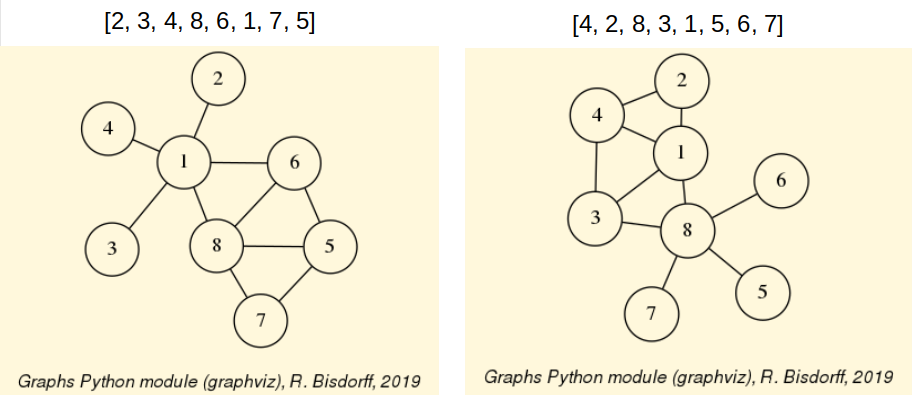
\includegraphics[width=10cm]{Figures/isomorphicPerms.png}
\caption{Isomorphic permutation graphs.} 
\label{fig:25.11}       % Give a unique label
\end{figure}

And, we indeed recover in Fig. \ref{fig:25.11} indeed two isomorphic copies of the original random graph (compare with Fig. \ref{fig:25.8}).
 
%%%%%%% The chapter bibliography
%\normallatexbib
\clearpage
%\phantomsection
%\addcontentsline{toc}{section}{Chapter Bibliography}
\bibliographystyle{spbasic}
%\typeout{}
\bibliography{03-backMatters/reference}
%\input{02-mainMatters/25-chapterPerfectGraph3.bbl}